%Tarea 2
\documentclass[10pt, oneside]{book}
\usepackage[utf8]{inputenc}
\usepackage[spanish]{babel}
\spanishdatedel
\usepackage{graphicx,float}%[demo]
\usepackage[usenames, dvipsnames, x11names, table, svgnames]{xcolor}
\usepackage{libertine}
\usepackage[libertine]{newtxmath}
\usepackage[scaled=.92]{sourcesanspro}
\usepackage[scaled=.78]{beramono}
\usepackage[protrusion=true, expansion = true]{microtype}
%\newcommand*{\sbdefault}{sb}
%\DeclareRobustCommand{\sbseries}{%
%\not@math@alphabet\sbseries\relax
%\fontseries\sbdefault\selectfont
%}
\usepackage{lipsum}
\usepackage{lscape}
\usepackage{tikz}

\usepackage[left = 2.5cm, right = 1cm, top = 3cm, bottom =1cm, foot = 5mm, head =1.5cm, width = 10cm, includeheadfoot]{geometry}
%\author{Oromion}
%\title{Lección V2.2}

\begin{document}
	%\maketitle
	\begin{titlepage}
		\newgeometry{hmargin = {1.5cm}, vmargin = {2cm}, nomarginpar, ignorefoot, ignorehead}
		\center
		\begin{large}
			\Huge{Growth of the number of simple closed geodesics on hyperbolic surfaces}
		\end{large}
		
		\vspace{2.5cm}
		
		\LARGE{Princeton University}\\
		\large{Department of Mathematics}
		
		\vspace{5mm}
		
		
\includegraphics[scale=.9]{1}
		
		\vspace{3cm}
		
		\begin{minipage}{.5\textwidth}
			Author: Maryam Mirzhakani\\
		\end{minipage}
		\hfill
		\begin{minipage}{.45\textwidth}
			\flushright
			Journal: Annals of Mathematics\\
			Pages: 97-125.
		\end{minipage}
		
		\begin{figure}[H]
			\centering
			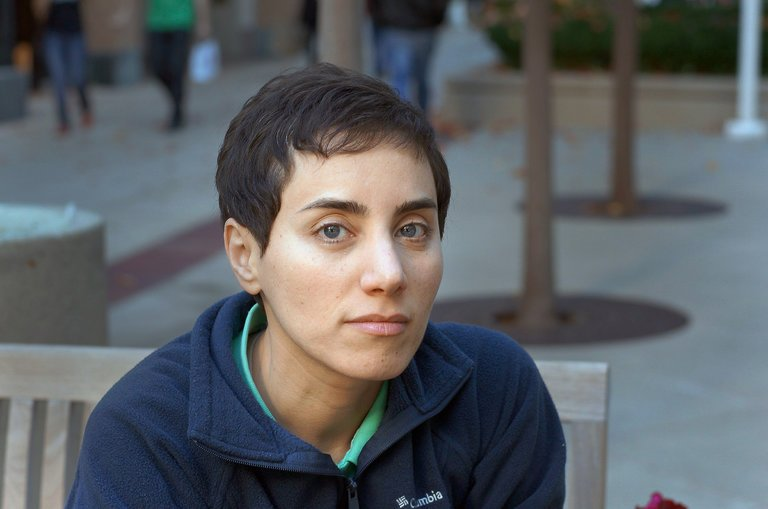
\includegraphics[scale=.2]{Mirzakhani.jpg}
		\end{figure}
		
		\vspace{2.5cm}
		
		\huge{2008}
	\end{titlepage}
	
\end{document}